% =====================================================================
% SWAT+ ENGINE ACCELERATION — manuscript (journal-agnostic skeleton).
% Venue: Computers & Geosciences.
% Compile from publication/engine-acceleration/manuscript:
%   pdflatex main && bibtex main && pdflatex main && pdflatex main
% Status: submission-ready (Computers & Geosciences).
% =====================================================================
\documentclass[12pt]{article}

% Shared preamble — SWAT+ engine-acceleration manuscript.
\usepackage[margin=1in]{geometry}
\usepackage{setspace}
\usepackage{graphicx}
\usepackage{booktabs}
\usepackage{array}
\usepackage{tabularx}
\usepackage{ragged2e}
\usepackage{longtable}
\usepackage{natbib}
\usepackage{amsmath}
\usepackage{listings}
\usepackage{xcolor}
\usepackage[hidelinks]{hyperref}
\usepackage{url}

\DeclareRobustCommand{\path}[1]{\nolinkurl{#1}}

\newcolumntype{Y}{>{\RaggedRight\arraybackslash}X}

\graphicspath{{../figures/}}

% Lightweight code listing style for the Fortran snippets (threadprivate, wavefront).
\lstdefinestyle{swxcode}{
  basicstyle=\ttfamily\small,
  keywordstyle=\color{blue!60!black},
  commentstyle=\color{green!40!black}\itshape,
  breaklines=true,
  frame=single,
  framesep=4pt,
  showstringspaces=false,
  language=Fortran,
}
\lstset{style=swxcode}

% Inline TODO marker for the drafting phase (strip before submission).
\newcommand{\TODO}[1]{\textcolor{red}{[\textbf{TODO:} #1]}}

% Headline parallel/total numbers (final engine, dedicated c8a AWS instance; consistent re-run).
\newcommand{\parHead}{5.33}    % peak self-relative thread speedup (c8a, N=24, still climbing)
\newcommand{\parHeadN}{24}     % thread count at that peak
\newcommand{\totHead}{7.14}    % combined stock->parallel total on c8a at 24 threads
\newcommand{\totMinutes}{half a minute} % per-year wall after parallelization (27 s on c8a)

% Figure placeholder: keeps the manuscript compiling before the image files exist.
% Swap \figplaceholder{...} for \includegraphics{...} once the figure is generated.
\newcommand{\figplaceholder}[2]{%
  \fbox{\begin{minipage}[c][3.2cm][c]{0.88\textwidth}\centering
    \textcolor{red}{\textbf{[FIGURE TO GENERATE: \texttt{#1}]}}\\[4pt]
    \textcolor{red}{\footnotesize #2}
  \end{minipage}}%
}

\usepackage{lineno}

\doublespacing
\linenumbers

\title{Accelerating a Regional Hyper-Resolution {SWAT+} Model Without Changing the Science:
a Reproducible Profiling-to-Parallelization Methodology and a Routing-Aware
Shared-Memory Wavefront}

\author{%
  Vahid Rafiei\\
  Independent Researcher\\
  \texttt{vahidr32@gmail.com}\\
  ORCID: \href{https://orcid.org/0009-0009-8309-1895}{0009-0009-8309-1895}
}

\date{}

\begin{document}

\maketitle

\begin{abstract}
\noindent
Process-based watershed models such as SWAT+ are increasingly applied at regional,
hyper-resolution scale, where a single simulation becomes the bottleneck: one simulated year of a
57{,}998-hydrologic-response-unit (HRU) model takes about three minutes on one core,
and calibration multiplies that by thousands of evaluations. Existing parallel SWAT efforts exploit
ensemble parallelism (many independent runs) or grid-cell decomposition; the cost of a single
simulation is left untouched. We present a reproducible methodology for accelerating the SWAT+
engine itself on shared-memory hardware without altering model results: profile, classify the
bottleneck, fix by class, validate, re-measure. Profiling shows the dominant costs at scale are
overhead, not hydrology---per-object array re-zeroing, derived-type copies, $\mathcal{O}(N^2)$
name-matching, and a serial routing critical path. We remove these and add an OpenMP
parallelization that respects the routing directed acyclic graph: a topological level wavefront over
the engine's command order, made reentrant by privatizing current-object state. The result
separates two products: serial overhead removal accelerates the engine everyone already runs on one
core ($1.67$--$2.47\times$ across CPUs, no threads), while parallelization adds scaling for
many-core runs (up to \parHead$\times$ at \parHeadN{} threads, \totHead$\times$ over the stock
single-core engine). Correctness is enforced by thread-count invariance---identical output across
thread counts---used as an automatable data-race detector. At one thread the engine is
byte-identical to the unmodified serial engine; at higher counts, exercising in-stream water quality
exposed a compiler-induced data race in particulate constituents ($15$--$20\%$ on three
sediment-associated species), which we resolve by a byte-identical land-parallel, routing-serial
mode. Strikingly, the single largest speed gain came not from threads but from removing one
redundant array reset on the serial main stem---a serial fix that also raised the parallel ceiling.
All code, every optimization as an individually validated commit, and the benchmark harness are
released.
\end{abstract}

\noindent\textbf{Keywords:} SWAT+; shared-memory parallelism; OpenMP; river routing;
reproducibility; model acceleration.


\section{Introduction}\label{sec:intro}
The Soil and Water Assessment Tool (SWAT) and its restructured successor SWAT+
\citep{Arnold1998SWAT,Bieger2017SWATPlus} are among the most widely used process-based
watershed models. As input data and computing have improved, the community has pushed SWAT+
toward larger domains and hyper-resolution discretizations---tens of thousands of
hydrologic response units (HRUs) and channels in a single basin. At that scale the cost of a
\emph{single} simulation becomes the binding constraint. The benchmark model used throughout
this paper, a USGS HUC-8 watershed (hydrologic unit 03100101) is a regional, hyper-resolution model
generated by the SWATGenX platform; it contains 57{,}998 HRUs and 8{,}181 channels (full
specification in Section~\ref{sec:model}), and one simulated year takes about three minutes on
a single core. Calibration---the dominant computational activity in practice---requires
hundreds to thousands of such evaluations, so per-run cost multiplies directly into days of
wall-clock time and substantial cloud expense.

\subsection{The gap: engine-level vs ensemble-level parallelism}
Most prior work on ``parallel SWAT'' accelerates the \emph{calibration}, not the
\emph{model}. Frameworks distribute independent parameter sets across cores or cluster nodes
\citep{Rouholahnejad2012Parallelization,Zhang2013Multiobjective,Yalew2013Grid}, and more
recent efforts containerize the same ensemble pattern for reproducibility
\citep{PASS4SWAT2024}. This ensemble parallelism is essential and we use it, but it has a
hard ceiling: population-based calibration of a model with a few tens of adjustable
parameters saturates at a few tens of concurrent evaluations \citep{Rafiei2022Calibration}---beyond
that, a larger population does not improve the optimum and can degrade it. Once an individual model
is large,
the only way to apply more than that handful of cores to \emph{one} model is to parallelize
the engine itself.

Engine-internal parallelization of SWAT is comparatively rare and has targeted the
embarrassingly parallel land phase: OpenMP over HRUs in the gridded SWATG variant
\citep{Zhang2017SWATG} and compiler-assisted OpenMP in SWAT \citep{Ki2015OpenMPSWAT}. The
land phase is the easy half. The hard half---channel routing---is a strictly ordered
traversal of the river network: a reach cannot be solved until its upstream contributors
are. This data dependency is exactly what makes routing the serial bottleneck, and it is the
same structural obstacle faced by every distributed routing model
\citep{David2011RAPID,Mizukami2021mizuRoute,Yamazaki2011CaMaFlood}.

\subsection{Two non-negotiable constraints}
A parallel engine intended for real use must satisfy two constraints that the existing
literature largely sidesteps. First, results must not change: a calibrated,
published, or regulatory model cannot silently produce different numbers because it ran on
more cores. Second, correctness must be demonstrable, not asserted---data races in
shared-memory scientific codes are notoriously intermittent and escape casual testing
\citep{Atzeni2016ARCHER}. We treat both as first-class: the one-thread path reproduces the
unmodified serial engine \emph{bit for bit}, and we validate the parallel paths by
\emph{thread-count invariance}, a per-output bitwise consistency criterion in the spirit of
ensemble consistency testing for Earth-system models \citep{Baker2015CESMECT}, which here
doubles as a precise race detector.

\subsection{Contributions}
This paper makes the following contributions:
\begin{enumerate}
  \item A reproducible acceleration methodology for a large process-based Fortran model:
        profile $\rightarrow$ classify $\rightarrow$ fix-by-class $\rightarrow$ validate
        $\rightarrow$ re-measure, with each optimization an independently validated commit.
  \item A bottleneck taxonomy of SWAT+ at scale, with the central empirical finding
        that the dominant cost is \emph{overhead, not hydrology}---per-object array zeroing,
        struct copies, $\mathcal{O}(N^2)$ name lookups, and a serial routing critical path.
  \item A routing-DAG-aware shared-memory parallelization: a topological level
        wavefront over the engine command order, with reentrancy achieved by privatizing
        current-object state (\texttt{threadprivate}), and a discussion of the
        Fortran \texttt{SAVE}-locals hazard that makes na\"ive privatization unsafe.
  \item A correctness framework: byte-identity at one thread plus thread-count
        invariance as an automatable race detector, and an honest accounting of a compiler-induced
        in-stream particulate race ($15$--$20\%$ on three sediment-associated species) and its
        resolution by a byte-identical mode.
  \item An architectural-limit result: a measured characterization of where the
        SWAT+ daily step is parallelizable (the wide land phase) and where it is bound by the
        converging main-stem critical path, validated across multiple CPU microarchitectures.
\end{enumerate}

The remainder of the paper reviews related work (Section~\ref{sec:related}), details the
methodology and the parallelization (Section~\ref{sec:methods}), reports scaling and
correctness results (Section~\ref{sec:results}), and discusses the architectural limits and
portability (Sections~\ref{sec:discussion}--\ref{sec:conclusions}).


\section{Related work}\label{sec:related}
We organize prior work along the axis that matters for this paper: \emph{where} the
parallelism is extracted. Three layers are distinguishable---ensemble (many independent
runs), spatial-domain decomposition (split the watershed), and engine-internal
(parallelize one run's daily step)---and the serial routing dependency reappears as the
central obstacle at every layer.

\subsection{Ensemble-level parallelism for calibration}
The most mature line of work parallelizes the \emph{calibration loop} rather than the model.
\citet{Rouholahnejad2012Parallelization} introduced a parallelization framework for SWAT
calibration (the basis of the widely used SWAT-CUP workflow), distributing independent
parameter sets across cores. \citet{Zhang2013Multiobjective} coupled SWAT to a Python
parallel layer (mpi4py/OpenMPI) driving a multi-objective evolutionary optimizer, reporting
ensemble speedups of 45--109$\times$ on a cluster depending on model complexity.
\citet{Yalew2013Grid} parallelized a large spatially distributed model via MPI, and
\citet{PASS4SWAT2024} recently containerized the calibration ensemble for computational
reproducibility. These approaches are complementary to ours and remain the right tool for
exploring parameter space. Their limitation is structural: population-based search over a
model with $\sim$tens of parameters saturates at $\sim$tens of concurrent evaluations, so
ensemble parallelism cannot reduce the wall-clock cost of an \emph{individual} large
simulation, nor apply more than that handful of cores to a single model. That is precisely
the regime this paper addresses.

\subsection{Engine-internal parallelism in SWAT/SWAT+}
Fewer studies parallelize the SWAT engine itself, and those that do concentrate on the land
phase, which is embarrassingly parallel across HRUs. \citet{Ki2015OpenMPSWAT} applied
Intel-compiler OpenMP to SWAT and benchmarked the result; \citet{Zhang2017SWATG} added OpenMP
over HRUs to the gridded SWATG variant (``SWATGP''), reporting up to $\sim$9$\times$ on a
$\sim$2000~km$^2$ watershed at 500~m with 15 threads. Two observations motivate our work.
First, these efforts parallelize the land phase but do not tackle the channel-routing
critical path, which our profiling (Section~\ref{sec:results}) shows is roughly $7\times$ the
land-phase cost on a large basin---so land-phase-only speedup is Amdahl-bounded by the
serial routing remainder. Second, the SWAT+ restructuring \citep{Bieger2017SWATPlus}
replaced subbasins with an object/command architecture, which changes the parallelization
problem from ``loop over HRUs'' to ``traverse a heterogeneous object DAG''; to our knowledge
a routing-DAG-aware shared-memory parallelization of SWAT+ that preserves bit-level results
has not been reported.

\subsection{The serial routing dependency in other hydrological models}
The obstacle we confront---downstream reaches depend on upstream outflow---is fundamental to
river routing and has shaped the design of every continental routing model. The strategies
divide cleanly:
\begin{itemize}
  \item \textbf{Matrix linearization (solve all reaches at once).} RAPID
        \citep{David2011RAPID} casts Muskingum routing on a vector network into a single
        sparse linear system per time step and solves it with a parallel linear-algebra
        backend (PETSc), turning the topological dependency into matrix structure. This
        scales but requires a linear routing scheme and a global solve.
  \item \textbf{Spatial-domain decomposition.} mizuRoute
        \citep{Mizukami2021mizuRoute} partitions the network into sub-basins with a two-level
        hierarchical decomposition for distributed-memory (MPI) execution, and---in its
        impulse-response mode---parallelizes primarily in the \emph{time} dimension while
        preserving sequential topological order. CaMa-Flood \citep{Yamazaki2011CaMaFlood}
        partitions the global domain into subdomains and advances local inertial equations,
        updating cells in parallel across space. A recent study parallelizes channel routing
        by straightforward domain decomposition of the network \citep{Liu2023DomainDecompRouting}.
\end{itemize}
These are predominantly \emph{distributed-memory} designs that either change the numerics
(linearization) or partition the domain across ranks (decomposition), and they generally do
not guarantee bitwise identity to a serial reference. Our setting differs in three ways: we
keep SWAT+'s existing (nonlinear, sub-stepped) routing numerics unchanged; we target
\emph{shared}-memory many-core nodes (the common cloud-calibration unit) rather than clusters;
and we make preservation of the serial result a hard requirement. Our mechanism---a
topological \emph{level wavefront} that runs all DAG nodes at the same depth concurrently and
synchronizes between levels---is the shared-memory analogue of the dependency-respecting
ordering those models implement across ranks.

\subsection{Correctness and reproducibility of parallel scientific code}
Shared-memory parallelization of a large mutable-state Fortran model is dominated by the risk
of data races, which are intermittent and poorly exposed by ordinary testing
\citep{Atzeni2016ARCHER}. Dynamic and static race detectors exist but scale awkwardly to a
model of SWAT+'s size and global-state idioms. We instead adopt an output-level criterion:
\emph{thread-count invariance}, requiring repeated runs at different thread counts to produce
identical daily output. This is conceptually aligned with the ensemble-consistency testing
used to certify Earth-system-model ports across compilers and machines
\citep{Baker2015CESMECT}, but applied at bit granularity and used \emph{diagnostically}---a
run-to-run difference localizes the exact unprotected state. We also separate genuine races
from benign floating-point non-associativity introduced by aggressive compiler optimization
(\texttt{-ipo}); the latter is a known source of bit-level variation \citep{IntelOneAPI} and
is quantified rather than conflated with incorrectness.


\section{Methods}\label{sec:methods}
\subsection{Benchmark model and toolchain}\label{sec:model}
All measurements use a single benchmark model so that speedups are comparable across
optimizations: a single USGS HUC-8 watershed (hydrologic unit 03100101; the Peace River, southwest Florida), a
\emph{regional, hyper-resolution} SWAT+ model generated by the SWATGenX platform. The basin is
delineated from the USGS National Hydrography Dataset Plus High Resolution (NHDPlus~HR) over a
$1/3$~arc-second ($\approx$10~m) DEM, with land cover from the 500~m National Land Cover Database
(NLCD), soils from gridded SSURGO (gSSURGO), and climate forcing from PRISM (precipitation and
temperature) and the National Solar Radiation Database (NSRDB). The model comprises
57{,}998 hydrologic response units (HRUs), 8{,}181 channels, 9{,}341 routing units
(subbasins) resolved into 9{,}342 landscape units, 326 reservoirs and lakes, and 170 aquifers.
The high HRU count follows from the large drainage area combined with a hyper-resolution
slope/land-cover/soil intersection---this is a single regional model, not a continental one,
though the SWATGenX platform provides model-building coverage across the conterminous United
States (CONUS). Unless stated otherwise, the timed workload is one simulated year, which exercises
the full daily land-and-routing step over the entire network. The engine is built with the Intel
oneAPI Fortran compiler (\texttt{ifx}) at \texttt{-O3 -ipo}; \texttt{gfortran} fails to produce a
working binary at this model size, so \texttt{ifx} is the reference toolchain. OpenMP is enabled
with \texttt{-fiopenmp}. We keep two binaries---the unmodified serial engine and the parallel
engine---so the parallel work can be checked against an exact reference; at one thread the
parallel engine executes the original serial code path (Section~\ref{sec:validation}).

\subsection{The acceleration loop}
The methodology is a disciplined iteration, applied until returns diminish:
\begin{enumerate}
  \item \textbf{Profile.} Intel VTune \texttt{hotspots} collection on a representative window
        (180 simulated days), reported per routine and per source line, to find where time is
        actually spent rather than where it is assumed to be spent.
  \item \textbf{Classify.} Assign each hotspot to a class---startup name-matching, per-object
        re-initialization, derived-type copies, serial critical path, or genuine hydrologic
        compute---because the fix differs by class and the classification is the transferable
        result.
  \item \textbf{Fix by class.} Apply the class-appropriate change (e.g.\ index a name lookup,
        scope an array reset, privatize shared scratch, restructure for parallelism).
  \item \textbf{Validate.} Re-run the correctness battery (Section~\ref{sec:validation})
        before accepting any change.
  \item \textbf{Re-measure.} Re-time and re-profile; the new dominant hotspot becomes the next
        target. Each accepted change is a single version-control commit whose message records
        its validation evidence.
\end{enumerate}

\subsection{The routing DAG and the level wavefront}\label{sec:wavefront}
SWAT+ advances one daily time step by walking every object---HRU, routing unit, channel,
reservoir, aquifer---in a single fixed sequence (the \emph{command order}). That sequence
encodes the river network's connectivity: an object appears after all objects that feed it.
Equivalently, the command order is a topological sort of a directed acyclic graph (DAG) whose
edges are the hydrologic routing connections.

A topological sort admits a \emph{level} (antichain) decomposition: level $\ell$ contains
every object all of whose upstream dependencies lie in levels $<\ell$. Objects within a level
are mutually independent and may be computed concurrently; levels must be processed in order.
We precompute this level index once per run from the command order and drive the daily step
as a level wavefront: for each level, an OpenMP parallel loop computes its objects; an
implicit barrier between levels preserves the upstream-before-downstream ordering. For the
benchmark network this yields 265 levels: level~1 is the entire land phase
($\approx$58{,}000 HRUs---an enormous wide level with abundant parallelism), and the levels
narrow as the channel network converges, reaching width~1 at the deep main-stem
reaches---the serial critical path that ultimately bounds the achievable speedup
(Figure~\ref{fig:levels}; Section~\ref{sec:discussion}).

\begin{figure}[t]
\centering
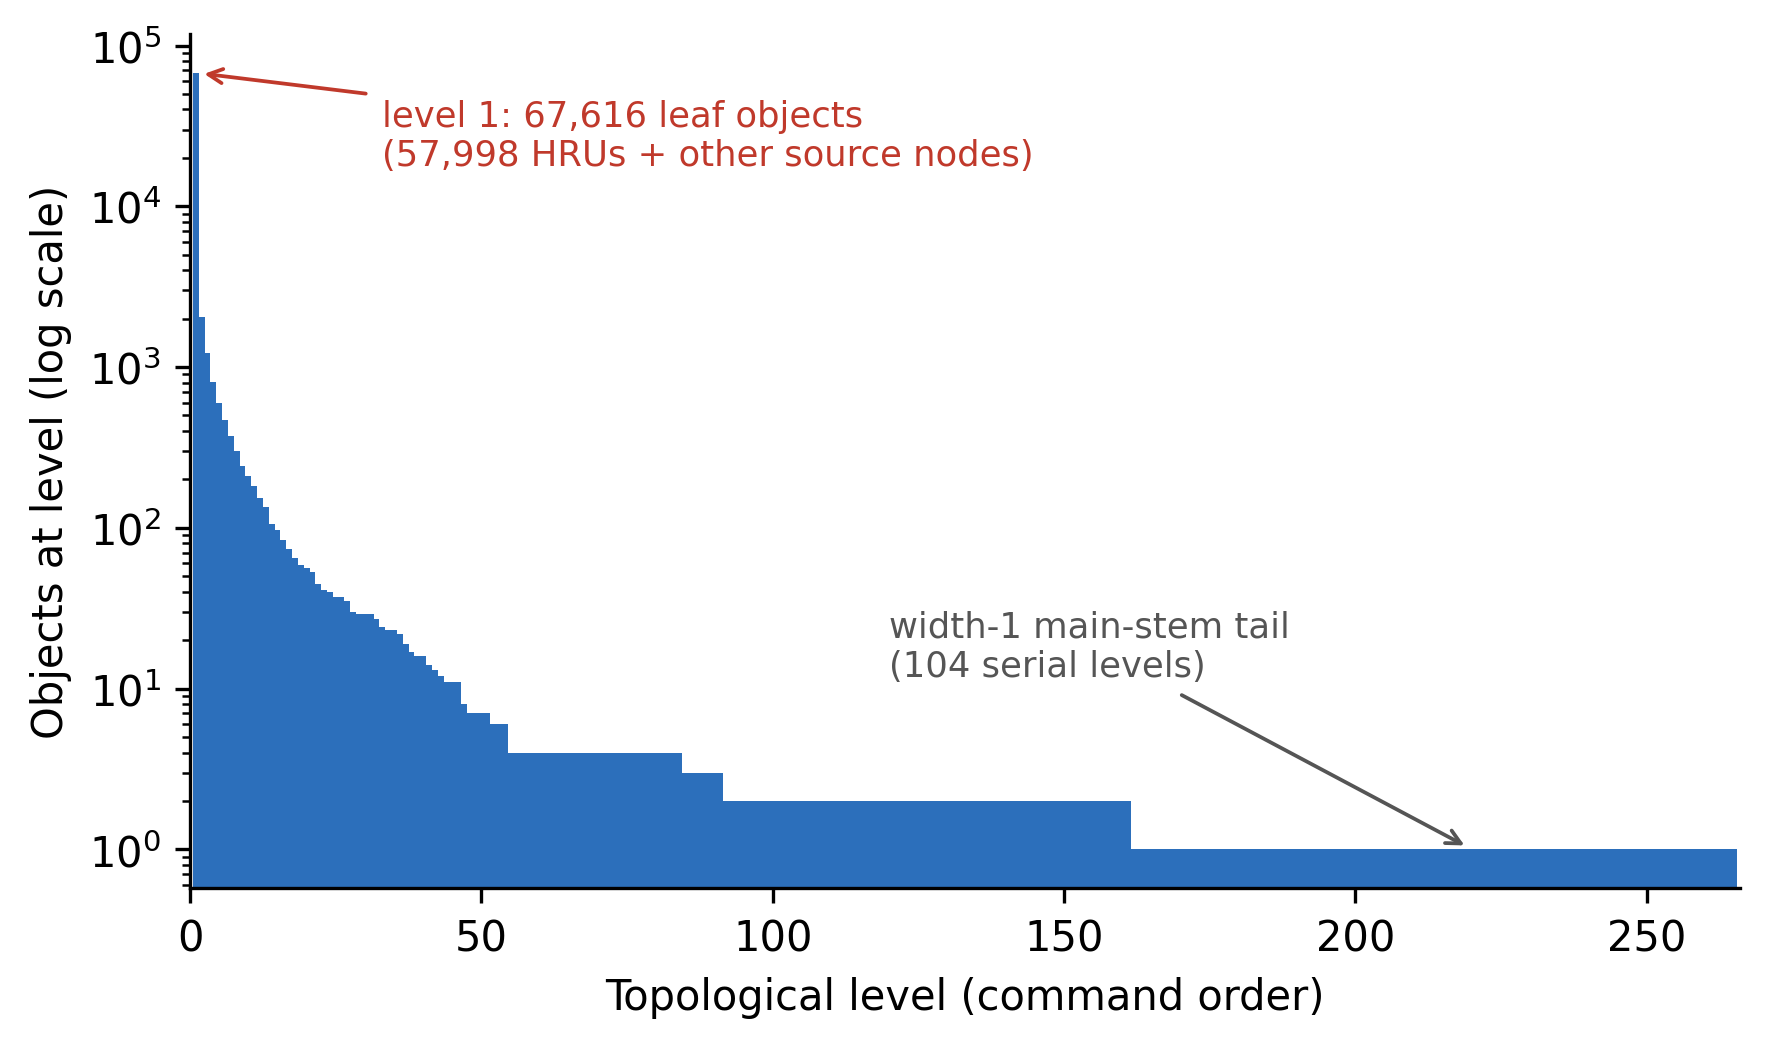
\includegraphics[width=0.78\textwidth]{Figure_1.png}
\caption{The command-order level decomposition for the benchmark river network (265 levels).
Level~1 contains all 67{,}616 objects with no upstream dependency---the 57{,}998 HRUs together with
the other source (leaf) nodes (point-source/recall objects and headwater units)---an enormously wide,
abundantly parallel level; the levels narrow monotonically as the channel network converges,
reaching width~1 at the deep main-stem reaches (104 successive width-1 levels). The length of this
width-1 tail, not the per-level synchronization, sets the Amdahl ceiling on single-run speedup
(Section~\ref{sec:discussion}).}
\label{fig:levels}
\end{figure}

Two engineering refinements proved necessary. First, forking a parallel region \emph{per
level} (265 times per day) made thread-management overhead dominate and caused an
\emph{8-thread regression}; we instead open one parallel region per simulated day and
drive the levels inside it, with the per-level barrier as the only synchronization. Second,
the long tail of width-1 (and other very narrow) levels paid one barrier each for almost no
parallel work; we fuse consecutive narrow levels into a single master-thread serial
block, so the deep main stem pays one barrier instead of one-per-level
(Figure~\ref{fig:wavefront}).

\begin{figure}[t]
\centering
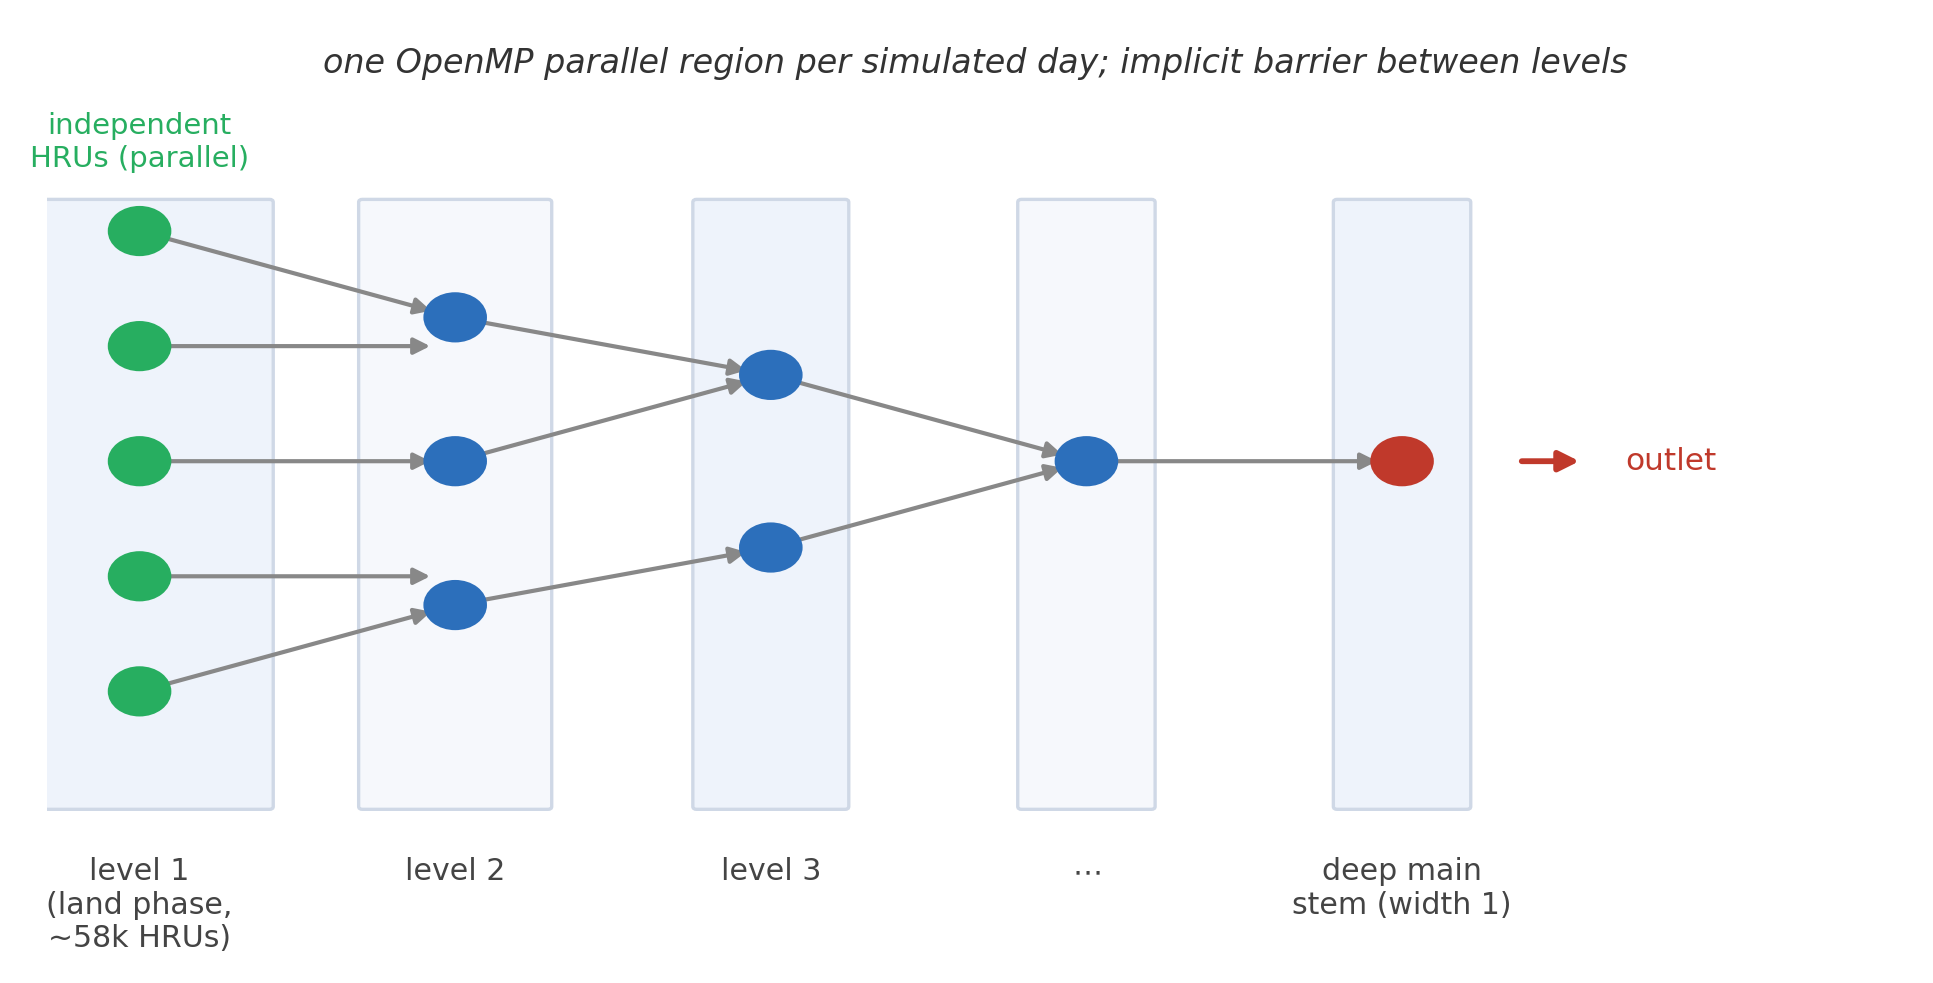
\includegraphics[width=0.82\textwidth]{Figure_2.png}
\caption{The routing-DAG level wavefront. The daily command order is a topological sort of the
routing DAG; objects at the same level are independent and run concurrently under a single
per-day OpenMP parallel region, with an implicit barrier between levels enforcing
upstream-before-downstream order. Consecutive narrow (near-width-1) levels on the main stem
are fused into one serial block to avoid paying a barrier per level. At one thread the
wavefront is inactive and the original serial command order executes unchanged.}
\label{fig:wavefront}
\end{figure}

\subsection{Reentrancy: privatizing current-object state}\label{sec:reentrancy}
The obstacle to running objects concurrently is not the routing math---it is that the engine,
though written in modern Fortran, communicates through \emph{module-global ``current-object''
scratch} by design: a routine sets a
global index (``the HRU we are on'', ``the channel we are on'') and downstream routines read
it. Under threads, concurrent objects clobber that shared state between the set and the use.
Making the per-object body reentrant therefore required auditing every such variable and
giving each thread its own copy via OpenMP \texttt{threadprivate}. Examples that had to be
privatized include the current weather-station index (a shared read of \texttt{iwst} between
its set and use caused $\sim$0.2\% PET drift on a station-dependent subset of HRUs), the
channel dispatch indices and rating-curve/peak-rate scratch, and a large cluster of
plant/residue ``temporary storage'' arrays.

A Fortran-specific hazard complicates this: a local declared with an initializer is
\emph{implicitly} \texttt{SAVE}d, hence shared across calls and therefore across threads, so the
reflexive ``strip the initializer'' fix is correct only for write-before-read scratch; the few
accumulators that legitimately persist must be kept \texttt{SAVE}d \emph{and} marked
\texttt{threadprivate}. This subtlety, and the one-thread byte-identity check that caught it, are
detailed in Supplementary Section~S2.

\subsection{Targeted hotspot removal (overhead, not hydrology)}\label{sec:hotspots}
Profiling repeatedly surfaced \emph{non-hydrologic} hotspots, each removed without touching the
science: an $\mathcal{O}(N^2)$ string name-match at startup (replaced by an $\mathcal{O}(1)$ index),
a per-object whole-array re-zeroing in the stream-temperature routine (\texttt{ch\_temp}, which
re-zeroed the entire landscape-unit array once per channel per day---the single hottest line in the
engine), and redundant derived-type struct copies in inflow-hydrograph handling. Each was scoped or
indexed to the data actually used, leaving output bit-identical; Section~\ref{sec:groupA} reports
the per-rung effect.

\subsection{Correctness framework}\label{sec:validation}
We validate with two complementary criteria.

\paragraph{Byte-identity at one thread.} At one thread the wavefront is inactive and the
engine executes the original command order, so its daily output must match the unmodified
serial engine \emph{bit for bit}. We verify this with exact byte-level diffs of every
daily HRU and channel record on a one-year benchmark run. This check caught a small
($\sim$0.3\%) \emph{deterministic} residual introduced by the reentrancy refactor in two
routines (\texttt{ch\_watqual4}, \texttt{et\_pot}), where stripping \texttt{SAVE} had dropped
persistent scratch values; restoring them as \texttt{threadprivate} \texttt{SAVE} state made
one-thread output bit-identical again (Section~\ref{sec:reentrancy}).

\paragraph{Thread-count invariance as a race detector.} For $N>1$ we require repeated runs at
different thread counts (1-vs-4, 4-vs-4, 4-vs-8) to produce identical daily output. Because a
correct shared-memory program is deterministic regardless of how work is scheduled, any
run-to-run difference is, by definition, a real data race---and the specific output fields
that differ point directly at the unprotected state. We use a strict tripwire (any record off
by $>10^{-6}$ counts as a difference). This criterion is what drove the iterative
race-elimination in Section~\ref{sec:reentrancy} and is fully automatable.

\paragraph{Separating compiler noise from incorrectness.} The \texttt{-ipo} production build
reorders floating-point operations, so two algorithmically identical builds can differ at the
last bits. We therefore distinguish (i) a non-\texttt{ipo} build, which is bit-identical to
the serial source and proves the \emph{algorithm} is unchanged, from (ii) the \texttt{-ipo}
build, whose residual ($\sim$$5\times10^{-4}$ relative, $\approx$0.008\%) is compiler
floating-point reassociation, not a logic change. Exercising the full process chain exposed one
$N>1$ data race in the in-stream \emph{particulate} constituents (Section~\ref{sec:correctness}),
localized to the channel constituent-transport path and under active resolution; hydrology and
dissolved species are model-equivalent across thread counts. The stream-temperature column is a
separate pre-existing upstream out-of-bounds read, output-only in the non-gwflow path, preserved
deliberately to match the reference serial behavior.


\section{Results}\label{sec:results}
We report results as a \emph{cumulative optimization ladder}: starting from the unmodified
stock engine, each optimization \emph{class} is added in a fixed order and its marginal
contribution measured on the same model, box, and protocol (Section~\ref{sec:methods},
Table~\ref{tab:ladder}). This isolates two qualitatively different products: Group~A
optimizations remove serial overhead and so benefit \emph{every} user on a single core with no
behavior change; Group~B (parallelization) benefits users who apply many cores to a
single model. All rungs---including the I/O rungs whose techniques were introduced in prior work \citep[the NetCDF backend and channel print filter, benchmarked there;][]{Rafiei2026SWATGenX}---are
re-measured here on the 57{,}998-HRU benchmark, because their prior figures were obtained on a
different (94k-HRU) model and do not transfer; this keeps the stock$\rightarrow$final
comparison internally consistent.

\begin{table}[t]
\centering
\caption{Cumulative optimization ladder on the HUC-8 benchmark model (57{,}998 HRUs, one simulated
year, \texttt{ifx -O3 -ipo}, dedicated c8a.8xlarge, best of two). Each rung adds one class;
``marginal'' is the speedup from the preceding rung, ``cumulative'' is versus stock. All $N{=}1$
except the final-engine parallel row (Group~B).}
\label{tab:ladder}
\begin{tabular}{llrrr}
\toprule
Rung & Class & Wall $N{=}1$ (s) & Marginal & Cumulative \\
\midrule
R0 \quad Stock engine                 & baseline          & 191.9 & 1.00$\times$ & 1.00$\times$ \\
\quad + hru\_read O(1) index          & serial: startup   & 185.4 & 1.03$\times$ & 1.03$\times$ \\
\quad + varinit per-row reset         & serial: per-step  & 171.0 & 1.08$\times$ & 1.12$\times$ \\
\quad + drop inflow struct copy       & serial: channel   & 137.6 & 1.24$\times$ & 1.39$\times$ \\
\quad + ch\_temp reset scope          & serial: channel   & 138.9 & 0.99$\times$ & 1.38$\times$ \\
R6 \quad + final (narrow-fuse, $N{=}1$) & serial: final   & 115.2 & 1.21$\times$ & \textbf{1.67$\times$} \\
\midrule
\multicolumn{5}{l}{\emph{Group~B --- parallelization of the final engine (dedicated AWS instances, Table~\ref{tab:crosshw}):}} \\
R6 \quad final engine, parallel        & parallel          & --- & \parHead$\times$ & \textbf{$\approx$\totHead$\times$} \\
\bottomrule
\end{tabular}\\[2pt]
\footnotesize\emph{Wall times: dedicated c8a instance, one simulated year, daily \texttt{channel\_sd}
output, best of 2. I/O (NetCDF backend, an extension from our fork \citep{Rafiei2026SWATGenX}, re-measured
here): stock text output 222.8\,s $\rightarrow$ NetCDF 196.8\,s ($1.13\times$). The Group~B factor is
the final engine's peak self-relative thread speedup (\parHead$\times$ at \parHeadN{} threads); the
combined stock-to-parallel $\approx$\totHead$\times$ is measured end-to-end against the stock engine
on the same machine (Table~\ref{tab:crosshw}, \S\ref{sec:configurator}).}
\end{table}

\subsection{Group~A: serial overhead removal (one core, every user)}\label{sec:groupA}
The Group~A rungs change \emph{no} model behavior and require \emph{no} threads; they make the
engine everyone already runs faster. The central empirical finding is that these gains are
large because the stock engine spends much of its time on \emph{overhead, not hydrology}:
\begin{itemize}
  \item \textbf{I/O.} Re-encoding output from text to a NetCDF backend (a fork extension benchmarked in the companion paper \citep{Rafiei2026SWATGenX}, re-measured here) cuts disk traffic: stock text output
        222.8~s $\rightarrow$ NetCDF 196.8~s, $1.13\times$ at $N{=}1$.
  \item \textbf{Startup name-matching (hru\_read).} HRU input was matched by an $\mathcal{O}(N)$
        linear name search, $\mathcal{O}(N^2)$ over the dataset; an $\mathcal{O}(1)$ index removes
        it, output-identical ($1.03\times$, 191.9$\rightarrow$185.4~s).
  \item \textbf{Per-step re-initialization (varinit).} A daily $\mathcal{O}(N_{\mathrm{hru}}^2)$
        whole-array \texttt{memset} in variable initialization was scoped to the current HRU's
        row ($1.08\times$, 185.4$\rightarrow$171.0~s).
  \item \textbf{Channel per-step overhead.} Removing a redundant inflow-hydrograph struct copy was
        the largest single serial step ($1.24\times$, 171.0$\rightarrow$137.6~s). The
        \texttt{ch\_temp} reset---the single hottest line in the engine, re-zeroing the
        \emph{whole} landscape-unit array once per channel per day---was scoped to the units each
        channel uses; notably this barely moves the \emph{serial} time ($0.99\times$,
        137.6$\rightarrow$138.9~s) because its real effect is on the \emph{parallel} critical path
        (Section~\ref{sec:groupB}: removing it from the serial main stem markedly raised the
        multi-thread ceiling by shrinking the Amdahl serial fraction). This split---a fix that is
        nearly free serially but decisive in parallel---is itself a finding.
\end{itemize}
Group~A headline ($N{=}1$, no threads): a cumulative $1.67\times$ over the stock engine
(191.9$\rightarrow$115.2~s) on the c8a reference node, a free acceleration for the entire existing
user base independent of whether they ever enable threads. Because these gains attack
memory-bound overhead, they are \emph{larger} on the more memory-starved parts---up to $2.47\times$
on the Intel ``Granite Rapids'' node (Table~\ref{tab:crosshw})---so $1.67\times$ is a
conservative floor.

\subsection{Group~B: parallelization (scaling a single model)}\label{sec:groupB}
On top of the serial-optimized engine, the routing-DAG level wavefront (Section~\ref{sec:wavefront})
adds thread parallelism. Because Group~A removed the dominant serial channel hotspot, the parallel
speedup is no longer suppressed by it: removing the \texttt{ch\_temp} reset on the critical path
shrinks the Amdahl serial fraction and so lifts the achievable scaling, and narrow-level fusion (one
barrier for the deep main stem instead of one-per-level) lifts it further. This interaction---a
serial fix raising the \emph{parallel} ceiling---is itself a result (Section~\ref{sec:discussion}).
All scaling is measured on quiet, dedicated AWS instances (one model per box, thread-pinned, best of
two); we report no shared- or contended-host timings.

\begin{table}[t]
\centering
\caption{Cross-hardware scaling of the final engine (each machine's own $1\rightarrow N$ ratio),
identical engine, one-simulated-year benchmark workload, daily \texttt{channel\_sd} output,
thread-pinned, best of two, on dedicated AWS instances. $t_1$ = one-thread wall on the parallel
binary. Boldface marks each CPU's peak; beyond it, threads land on SMT siblings and contend.}
\label{tab:crosshw}
\begin{tabular}{lccc}
\toprule
 & c8a (AMD EPYC & c8i (Intel Xeon & c5a (AMD EPYC \\
 & ``Turin'') & ``Granite Rapids'') & ``Rome'') \\
\midrule
physical cores (vCPU)           & 32 (32) & 16 (32) & 16 (32) \\
SMT                             & off (1 thr/core) & on (2 thr/core) & on (2 thr/core) \\
stock $R_0$ (s, $N{=}1$)        & 191.9 & 272.2 & 350.6 \\
serial gain ($R_0{\to}R_6$)     & 1.67$\times$ & 2.47$\times$ & 2.16$\times$ \\
$t_1$ (s, parallel binary)      & 143.1 & 130.1 & 202.5 \\
\midrule
2 threads     & 1.70$\times$ & 1.59$\times$ & 1.62$\times$ \\
4 threads     & 2.79$\times$ & 2.41$\times$ & 2.47$\times$ \\
8 threads     & 3.95$\times$ & 3.29$\times$ & 3.21$\times$ \\
12 threads    & 4.54$\times$ & 3.75$\times$ & 3.60$\times$ \\
16 threads    & 4.90$\times$ & \textbf{4.01$\times$} & \textbf{3.81$\times$} \\
20 threads    & 5.18$\times$ & 3.73$\times$ & 3.51$\times$ \\
24 threads    & \textbf{5.33$\times$} & 3.74$\times$ & 3.58$\times$ \\
\bottomrule
\end{tabular}
\end{table}

The scaling is bounded by \emph{physical cores and memory bandwidth}, not thread count: SWAT+ at
this scale is memory-bound, so once enough cores saturate the wide land-phase level, additional
cores only wait at the narrow routing levels, and parts regress onto SMT siblings past their
physical-core count (Figure~\ref{fig:scaling-crosshw}; Section~\ref{sec:discussion}).

\begin{figure}[t]
\centering
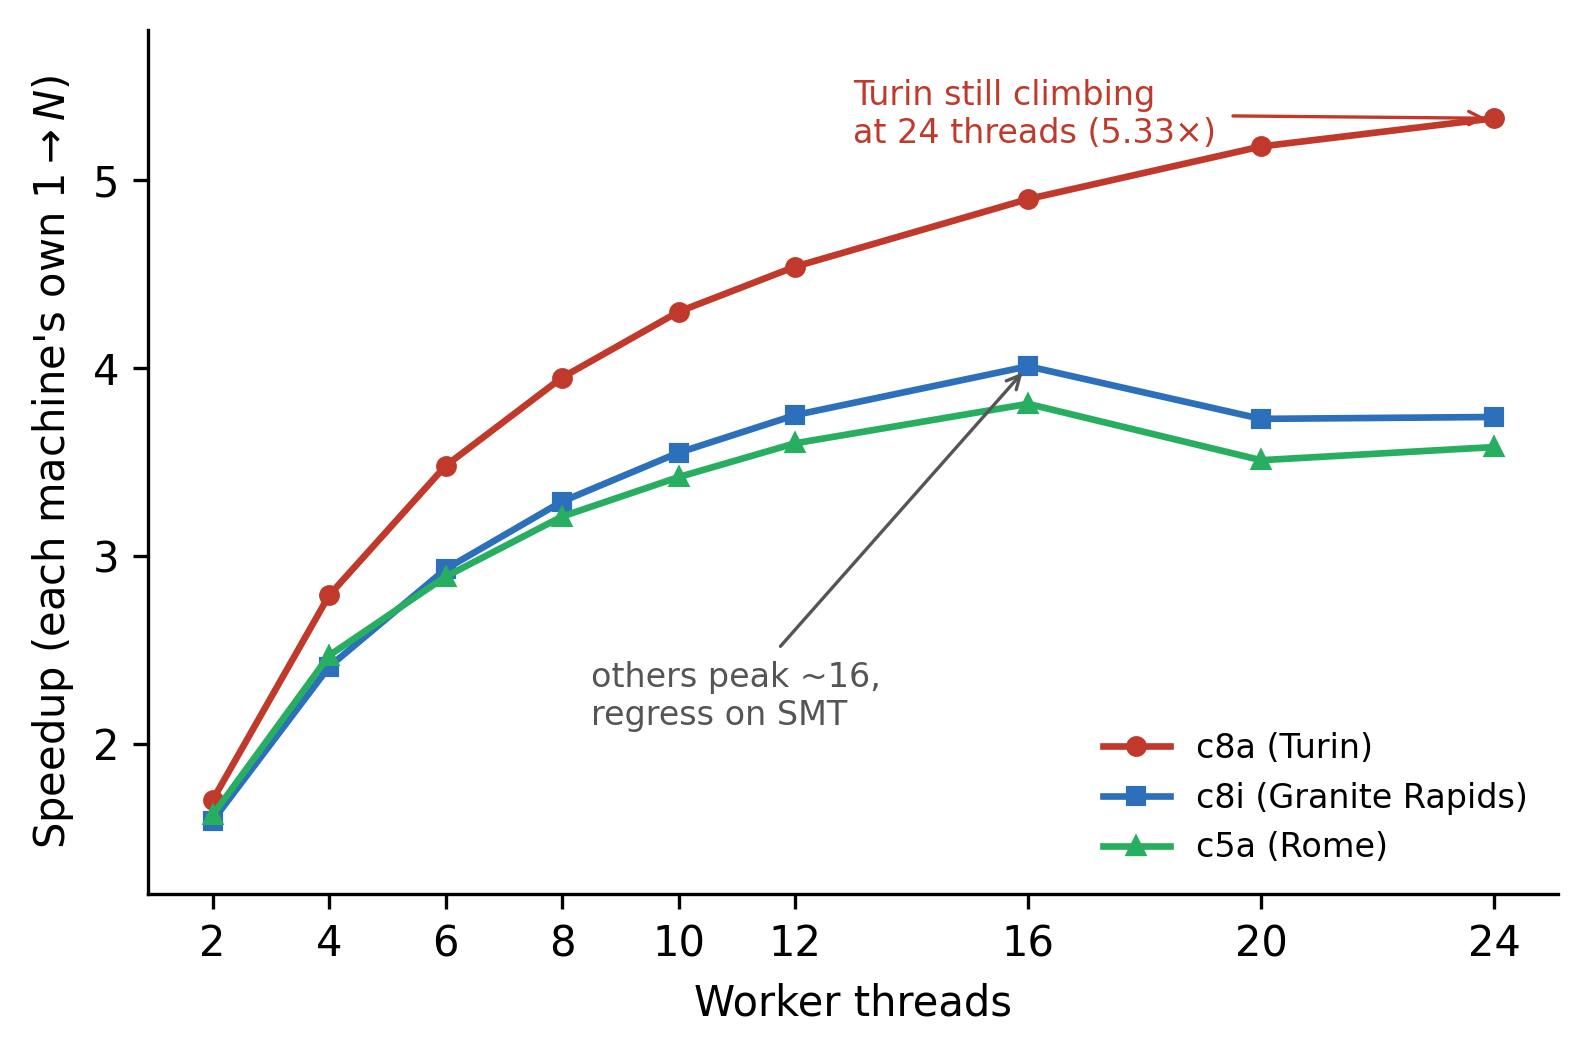
\includegraphics[width=0.78\textwidth]{Figure_3.png}
\caption{Cross-hardware scaling of the final engine on dedicated AWS instances. The workload is
memory-bound: speedup tracks physical cores and memory bandwidth, and parts regress once they run
onto SMT siblings.}
\label{fig:scaling-crosshw}
\end{figure}

\subsection{The bottleneck migrates across the campaign (VTune)}\label{sec:taxonomy}
Profiling at three points makes the campaign legible (Figure~\ref{fig:profile-triptych}). In the
\emph{stock} engine, channel routing and the to-be-removed overhead dominate; after Group~A, the
\texttt{ch\_temp} hotspot collapses (its hottest line falls from $\approx$731~s to
$\approx$0.8~s) and no channel routine is dominant; in the \emph{parallel} final engine at eight
threads, the bottleneck has migrated from computation to \emph{synchronization}---of the
$\approx$1{,}267 CPU-seconds the threads consumed, only $\approx$73\% is effective work,
$\approx$25\% is spin idling at level barriers while the serial main stem is walked, and
$\approx$2\% is overhead. The effective work that remains is dominated by serial channel
routing, which costs roughly $7\times$ the parallelizable land phase; the land phase is only
$\approx$12\% of compute, so the channel main stem---not more threads---is the remaining lever.

\begin{figure}[t]
\centering
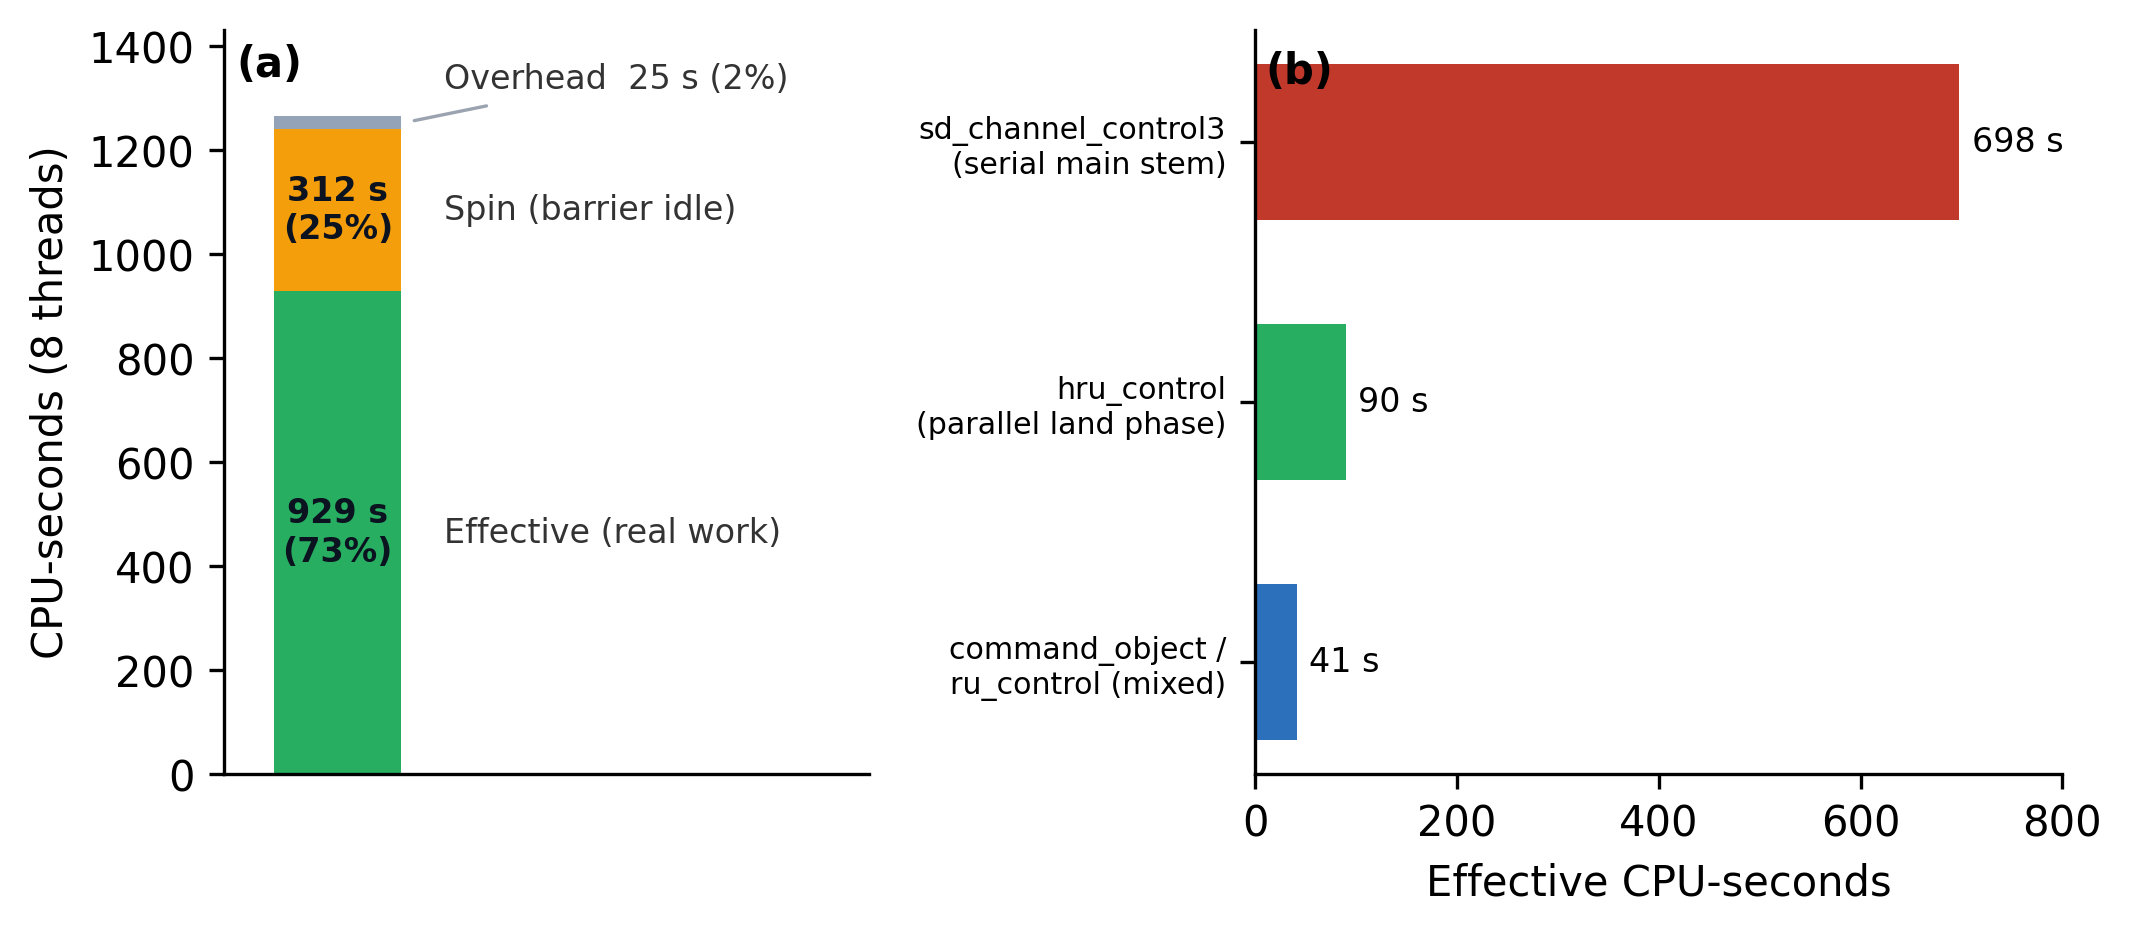
\includegraphics[width=0.92\textwidth]{Figure_4.png}
\caption{Intel VTune profile of the final engine at eight threads (180-day window).
\emph{(a)} CPU-time composition: only $\approx$73\% of the $\approx$1{,}266 thread-seconds is
effective work; $\approx$25\% is barrier spin idling against the serial main stem and $\approx$2\%
is scheduling/\texttt{threadprivate} overhead---the limit has migrated from computation to
synchronization. \emph{(b)} Effective work by routine: serial channel routing
(\texttt{sd\_channel\_control3}, 698~s) dominates the parallelizable land phase
(\texttt{hru\_control}, 90~s) by roughly $7.7\times$, so the main stem---not more threads---is the
remaining lever. (The Group~A serial pass earlier collapsed the dominant \texttt{ch\_temp} hotspot
from $\approx$731~s to $\approx$0.8~s; that hotspot is absent here.)}
\label{fig:profile-triptych}
\end{figure}

\subsection{Correctness: bit-identity at one thread; a localized particulate race at higher counts}\label{sec:correctness}
At one thread the parallel engine is byte-identical to the unmodified serial engine
(verified bit-for-bit on a one-year run), so an exact reference run is always available. At higher
thread counts, \emph{hydrology and
dissolved constituents are model-equivalent}: flow, sediment, nitrate, and soluble-phosphorus
basin loads agree to $<$2\% (mostly $<$0.5\%). The open item is the in-stream \emph{particulate}
constituents.

Reaching even this required treating \emph{thread-count invariance as a diagnostic} rather than a
checkbox (Section~\ref{sec:validation}) and exercising the full constituent chemistry: a
streamflow-only test passes while a latent race in the particulate constituents goes undetected.
Only with in-stream water quality active over a multi-year run does thread-count invariance expose a
$15$--$20\%$ divergence in three \emph{particulate/sediment-associated} species (organic-N, ammonia,
sediment-P), with run-to-run variation confirming a data race rather than reassociation. The HRU
land phase is byte-identical across thread counts and the dissolved species (NO$_3$, soluble-P) are
spared, localizing the race to the channel in-stream constituent-transport path.

\paragraph{Root cause (compiler, not algorithm).} ThreadSanitizer traces it not to a missing
\texttt{threadprivate}---every per-object buffer is privatized---but to \texttt{ifx} allocating the
\emph{temporaries} of the 152-byte \texttt{hyd\_output} derived type (operator results, function
returns, argument copy-ins) in shared static module storage rather than on the per-thread
stack, so concurrent channels clobber the same static temporary. The behavior is invariant to every
compiler control we tried, and a field-by-field source rewrite is byte-identical at one thread but
does not remove it (array-element arguments re-create static copy-in temporaries). The full forensic
trail is in Supplementary Section~S3.

\paragraph{Resolution: a byte-identical mode at a measured cost.} Because the race lives entirely in
the routing phase, running the land phase in parallel and the routing phase serially
(\texttt{SWATPLUS\_ROUTING\_SERIAL=1}) is race-free and byte-identical---thread-count-invariant to the
floating-point-reassociation floor. The cost is the routing phase's parallelism: the byte-identical
mode scales 2.04$\times$ at 4 threads / 2.50$\times$ at 8 versus the full wavefront's
2.79$\times$ / 3.98$\times$, a $\approx$37\% forfeit at eight threads that grows with thread
count (Supplementary Table~S3). The engine thus offers two modes: byte-identical for in-stream water
quality, and the full wavefront (bit-exact for flow/sediment/dissolved species) otherwise. A
non-\texttt{ipo} build is bit-identical to the serial source; the \texttt{-ipo} residual
($\sim$0.008\%) is reassociation, not the race.

\subsection{Putting it together: a speedup configurator}\label{sec:configurator}
Every speedup in this paper is measured against one fixed reference---the stock engine, one
thread, writing daily \texttt{channel\_sd} for all reaches---and the optimized and parallel runs
write the \emph{identical} output; we deliberately do not compare a fast filtered run against a slow
full-export run, which would fold an output-configuration choice into the engine number. The total
acceleration a practitioner sees is the product of three \emph{independent} layers, and conflating
them is the most common way these numbers are misread: (i)~output scope, an I/O effect
\emph{outside} the engine---full daily export of every object is several-fold slower than the
filtered calibration profile (of order $3$--$6\times$, growing with model size; companion study
\citep{Rafiei2026SWATGenX}) and is excluded from every figure here; (ii)~the machine-portable
serial gain ($1.67$--$2.47\times$, Group~A); and (iii)~the thread scaling above
(Group~B). Because the fixed-output baseline is already compute-bound, (ii) and (iii) compose on top
of (i). Figure~\ref{fig:configurator} shows the directly-measured stock$\rightarrow$parallel total on
the three CPUs plus the byte-identical mode; an interactive version is published with the open
engine, and the full layer composition is tabulated in Supplementary Section~S4.

\begin{figure}[t]
\centering
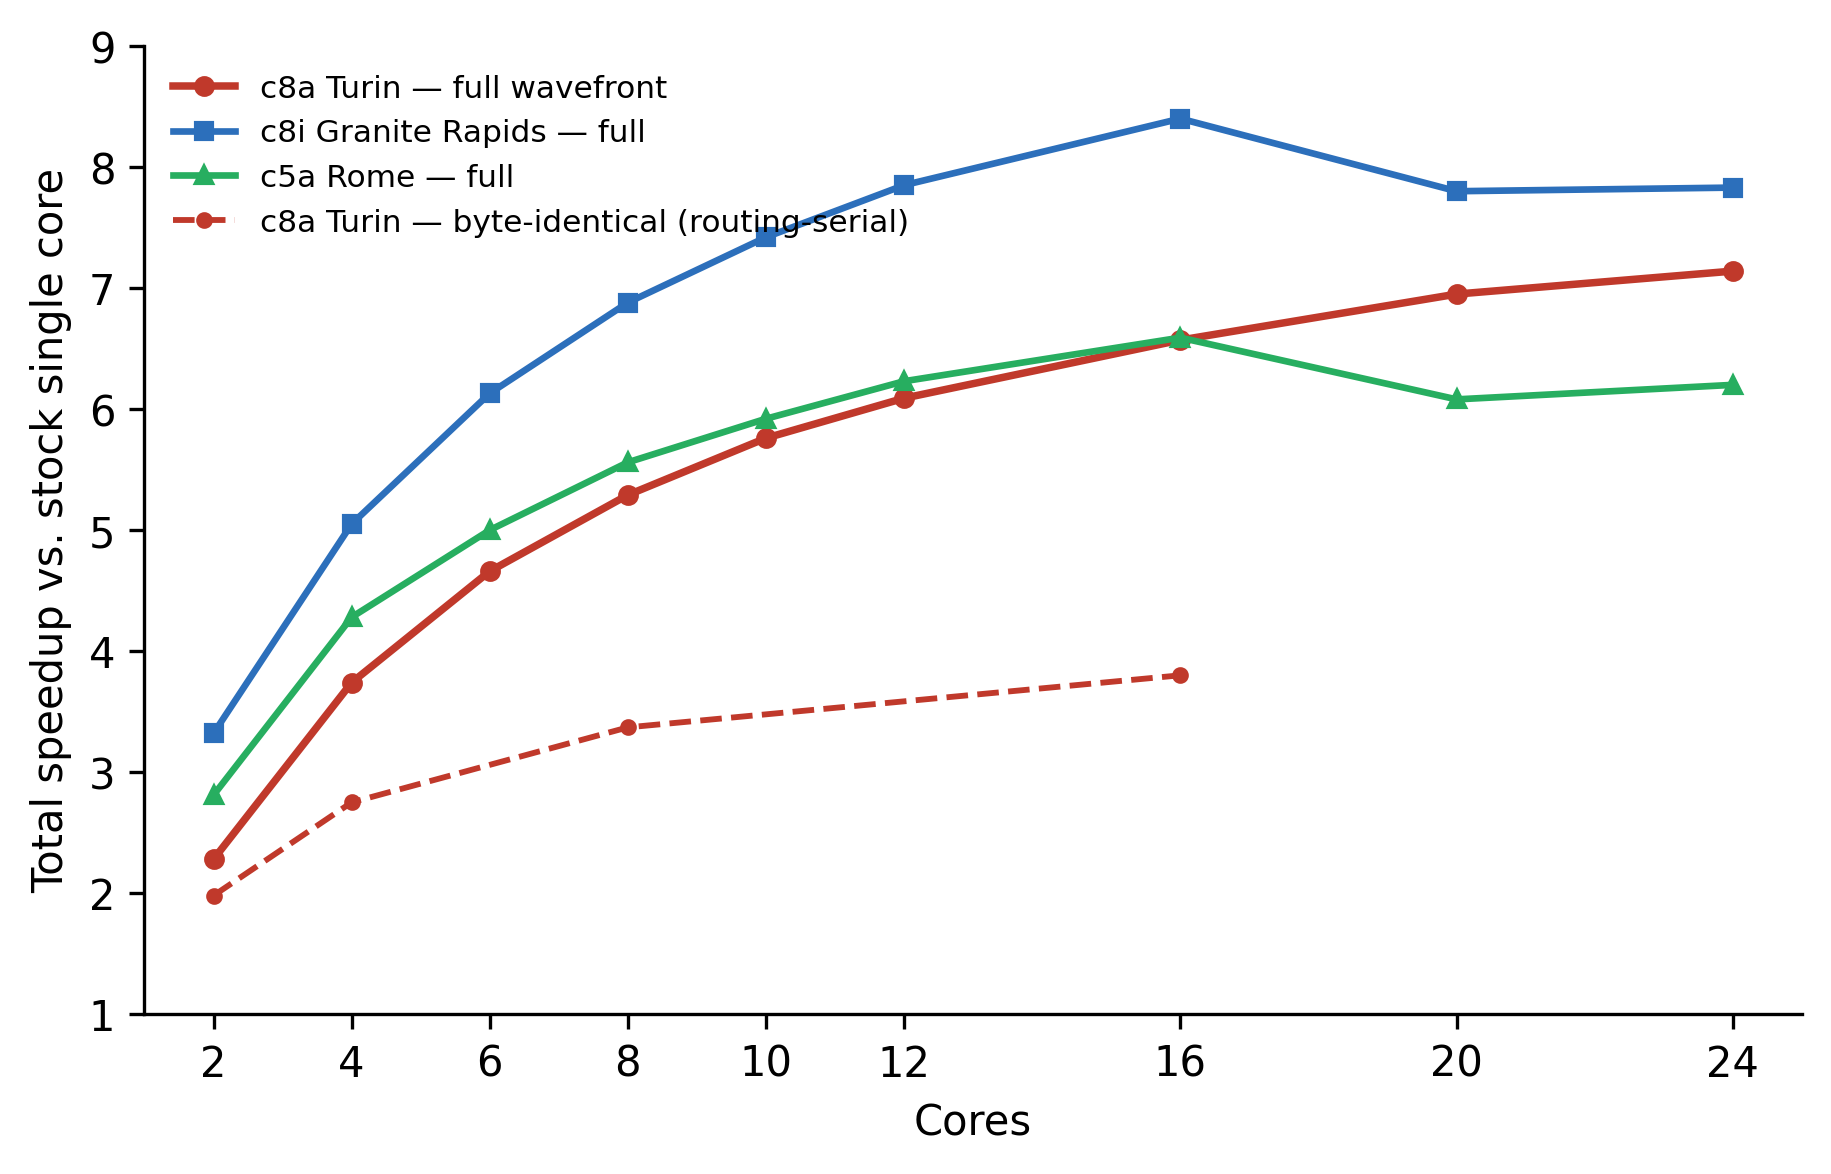
\includegraphics[width=0.82\textwidth]{Figure_5.png}
\caption{End-to-end engine speedup versus the stock single-core engine as a function of cores,
directly measured on three dedicated AWS CPUs (full wavefront), plus the byte-identical
routing-serial mode on the c8a node (dashed). The $1\times$ reference is the \emph{stock engine at
one thread writing daily \texttt{channel\_sd} for all reaches}; every curve writes that same output,
so the speedup is pure engine work, not reduced printing. Output-scope savings (layer~i; gauge
filtering, NetCDF) multiply on top and are deliberately excluded here.}
\label{fig:configurator}
\end{figure}

\subsection{Relevance to calibration}\label{sec:relevance}
Single-run acceleration is the lever that population-based calibration cannot otherwise reach.
Ensemble parallelism---running many independent evaluations concurrently---saturates at a few tens
of concurrent members \citep{Rafiei2022Calibration}, beyond which additional cores cannot help a
fixed population; accelerating the \emph{individual} simulation is then the only way to put more
cores on one model. The two contributions land differently here: the Group~A serial gains accelerate
every single evaluation with no threads and no behavior change, while the parallel engine lets a
calibration apply cores past the ensemble ceiling to each member.


\section{Discussion}\label{sec:discussion}
\subsection{Two products, cleanly separated}
The cumulative ladder (Table~\ref{tab:ladder}) deliberately separates two contributions that a
single blended speedup would conflate. Group~A---I/O reduction and serial overhead
removal---changes no model behavior and needs no threads, so it accelerates the engine
\emph{everyone already runs} and ships to all users through the default binary. Group~B
---the parallelization---benefits only those who put many cores on a single model. The
distinction matters for adoption: a practitioner on a laptop gains from Group~A for free, while a
practitioner calibrating a large basin on a many-core node additionally gains from Group~B. The
single most important practical message of this paper is that a large fraction of the
acceleration of the stock engine is achievable \emph{without parallelism at all}.

A cumulative ladder carries one caveat: a rung's marginal contribution depends on the order rungs
are added. We fix a logical order and report marginals \emph{given that order}; the cumulative
stock$\rightarrow$final factor is order-independent and is the headline number.

\subsection{A serial fix can raise the parallel ceiling}
The ladder also exposes an interaction that single-axis studies miss. The \texttt{ch\_temp}
reset is a Group~A (serial) fix, yet its largest visible effect was on \emph{parallel} scaling:
because it sat on the serial main-stem critical path, removing it shrank the serial fraction and
substantially lifted the multi-thread speedup ceiling. The lesson
is that on an irregular DAG with a long serial tail, serial-overhead removal and parallelization
are not independent---reducing critical-path work is often the most effective way to improve
parallel efficiency, more so than adding threads. This is why we measure each serial fix at
$N=1$ (its pure serial value) \emph{and} report its effect on the scaling curve.

\subsection{Where SWAT+ is parallelizable, and where it is not}
The scaling ceiling is not an implementation defect; it is the river network. The daily step
decomposes into a very wide land-phase level ($\approx$58{,}000 independent HRUs) followed by
a routing cascade that narrows monotonically to a width-1 main stem. By Amdahl's law
\citep{Amdahl1967} the achievable speedup is bounded by the serial fraction, and after the
\texttt{ch\_temp} fix that fraction is dominated by the \emph{length} of the converging
main-stem path---the 104 successive width-1 levels of Figure~\ref{fig:levels}---rather than by
per-level synchronization. This is visible in the cross-hardware
data: machines stop scaling at their physical-core count because, once enough cores exist to
saturate the wide levels, additional cores only wait at the narrow ones. The practical
implication is that for SWAT+, single-run acceleration past the land-phase regime requires
either (i) overlapping independent sub-trees of the routing DAG more aggressively across the
narrow levels, or (ii) reducing the per-channel arithmetic on the main stem (the in-stream
water-quality and sediment routines), not simply adding threads.

\subsection{Memory bandwidth, clock, and the meaning of ``speedup''}
SWAT+ at scale is memory-bound: the cross-hardware results show real cores beating
cores-plus-SMT and 32-core Turin out-scaling 16-core parts. Two reporting hazards follow.
First, hardware that turbo-boosts a single thread and down-clocks under load deflates the
$1\rightarrow N$ ratio, so the reported speedup understates the delivered parallel work. Second,
CPU-utilization monitors mislead---25\% of busy time at eight
threads was barrier spin, not work. We therefore report wall time and best-of-$N$ alongside
ratios, and we recommend the same discipline for comparable studies.

\subsection{Correctness as a methodology}
Treating thread-count invariance as the primary acceptance test, rather than spot-checking a
hydrograph, converted an open-ended race hunt into a localized, repeatable procedure in which each
failing output field named the unprotected state. It exposed two defects ordinary checks miss: an
implicit-\texttt{SAVE} Fortran initializer, and---only once in-stream water quality was exercised
over a multi-year run---a compiler-induced race in the particulate constituents
(Section~\ref{sec:correctness}). The transferable lesson is twofold: an equivalence test must
exercise the full process chain or it certifies only the subset it touches; and when a compiler will
not stack-allocate large derived-type temporaries, the safe granularity of shared-memory parallelism
is bounded by where those temporaries are shared.

\subsection{Portability and reproducibility}
The optimizations are standard OpenMP and portable Fortran; no machine-specific intrinsics are
used. The dependence on \texttt{ifx} reflects only that \texttt{gfortran} fails to build the
benchmark model at this size, not a hard requirement of the method. Every optimization is a
single commit carrying its own validation evidence, and the benchmark harness regenerates the
scaling tables, so the result chain is auditable end to end.

\subsection{Limitations}
The benchmark is a single (large) basin; while the bottleneck taxonomy should generalize to
any SWAT+ model with a deep routing network, the exact level histogram and the land-vs-channel
split are basin-specific, and small basins with shallow networks will see different ceilings.
The parallel path is validated for the non-gwflow configuration; the coupled groundwater
(\texttt{gwflow}) module is currently serial and disables the full-DAG wavefront, so
groundwater-surface-water runs do not yet benefit (a clearly scoped extension). Finally, the
cross-hardware study covers three microarchitectures but a single model size; a
size-vs-scaling sweep would strengthen the generality claim.


\section{Conclusions}\label{sec:conclusions}
We accelerated the SWAT+ engine on a regional, hyper-resolution HUC-8 benchmark (57{,}998
HRUs / 8{,}181 channels) without changing model results, reaching a measured \parHead$\times$
speedup at \parHeadN{} threads on a dedicated AMD ``Turin'' cloud node (about 3~min~$\rightarrow$
$\sim$\totMinutes{} per simulated year) and a combined $\approx$\totHead$\times$ over the stock
single-core engine. The central empirical result is that the dominant cost at scale is
\emph{overhead, not hydrology}: the single largest improvement came from removing one redundant
per-channel array reset on the serial critical path, not from adding cores. The parallelization is a
routing-DAG-aware shared-memory level wavefront over the engine command order, made safe by
privatizing current-object state, and its correctness is established by byte-identity to the serial
engine at one thread and by thread-count invariance---an automatable race detector---at higher
thread counts.

Methodologically, the contribution is a transferable loop for accelerating large process-based
scientific codes (profile $\rightarrow$ classify $\rightarrow$ fix-by-class $\rightarrow$
validate $\rightarrow$ re-measure) together with a bottleneck taxonomy and a correctness
framework that distinguishes genuine races from benign compiler floating-point reassociation.
Scientifically, the contribution is a precise characterization of where SWAT+'s daily step is
parallelizable (the wide land phase) and where it is architecturally serial (the converging
main-stem routing path), validated across multiple CPU microarchitectures. Because ensemble
calibration saturates at a few tens of concurrent members \citep{Rafiei2022Calibration},
accelerating the individual simulation is the only way to apply more cores to a single model. All
code, per-optimization commits, and benchmarks are released for reproduction and extension.


\section*{Code and data availability}
The SWAT+ engine fork, with every optimization as a separate commit carrying its validation
evidence in the commit message, is public at \path{https://github.com/rafiei-vahid/swatplus}. The
benchmark harness, the measured result files, the figure-generation script, and the benchmark model
(Peace River HUC-8 03100101, generated by the SWATGenX platform) are released at
\path{https://github.com/SWATGenX/swatplus-engine-acceleration}. The per-optimization commit map
and the build recipe are given in Supplementary Section~S1.

\section*{Acknowledgements}
Benchmark timings were obtained on dedicated Amazon Web Services (AWS) EC2 instances funded by the
author. The author thanks the SWAT+ developer community for the open engine on which this work
builds.

\section*{Author contributions}
V.R.\ designed the methodology, implemented the optimizations and parallelization, ran the
benchmarks, and wrote the manuscript.

\section*{Competing interests}
The author develops the SWATGenX model-generation platform, which deploys the engine described here;
no other competing interests are declared.

\bibliographystyle{plainnat}
\bibliography{../bib/references-engine}

\end{document}
